\documentclass{standalone}
\usepackage{tikz}
\usepackage{ctex,siunitx}
\setCJKmainfont{Noto Serif CJK SC}
\usepackage{tkz-euclide}
\usepackage{amsmath}
\usetikzlibrary{patterns, calc,3d}
\usetikzlibrary {decorations.pathmorphing,decorations.pathreplacing,decorations.shapes}
\begin{document}
\small
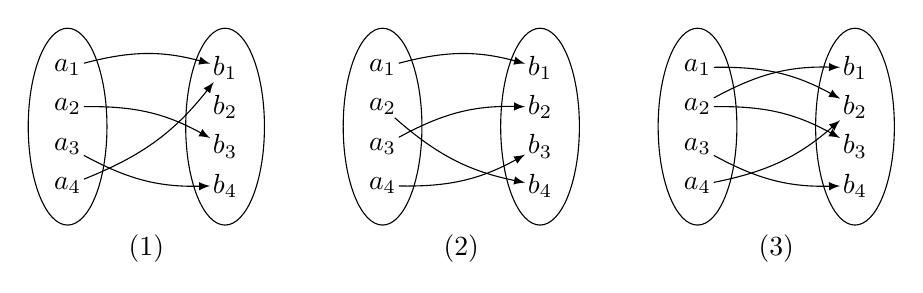
\begin{tikzpicture}[>=latex,scale=1.0,inner sep=1pt,outer sep=0pt]
  \begin{scope}
    \foreach \x in {1,2,3,4}
    {
      \node(a\x) at (-1,-0.5*\x){$a_\x$};
      \node(b\x) at (1,-0.5*\x){$b_\x$};
    }
    \draw(-1,-1.25)ellipse(0.5 and 1.25);
    \draw(1,-1.25)ellipse(0.5 and 1.25);
    \draw[->](a1)to[bend left=15](b1);
    \draw[->](a2)to[bend left=15](b3);
    \draw[->](a3)to[bend right=15](b4);
    \draw[->](a4)to[bend right=15](b1);
    \node at (0,-2.8){(1)};
  \end{scope}
  \begin{scope}[xshift=4cm]
    \foreach \x in {1,2,3,4}
    {
      \node(a\x) at (-1,-0.5*\x){$a_\x$};
      \node(b\x) at (1,-0.5*\x){$b_\x$};
    }
    \draw(-1,-1.25)ellipse(0.5 and 1.25);
    \draw(1,-1.25)ellipse(0.5 and 1.25);
    \draw[->](a1)to[bend left=15](b1);
    \draw[->](a3)to[bend left=15](b2);
    \draw[->](a2)to[bend right=15](b4);
    \draw[->](a4)to[bend right=15](b3);
    \node at (0,-2.8){(2)};
  \end{scope}
  \begin{scope}[xshift=8cm]
    \foreach \x in {1,2,3,4}
    {
      \node(a\x) at (-1,-0.5*\x){$a_\x$};
      \node(b\x) at (1,-0.5*\x){$b_\x$};
    }
    \draw(-1,-1.25)ellipse(0.5 and 1.25);
    \draw(1,-1.25)ellipse(0.5 and 1.25);
    \draw[->](a1)to[bend left=15](b2);
    \draw[->](a2)to[bend left=15](b1);
    \draw[->](a2)to[bend left=15](b3);
    \draw[->](a3)to[bend right=15](b4);
    \draw[->](a4)to[bend right=15](b2);
    \node at (0,-2.8){(3)};
  \end{scope}
\end{tikzpicture}
\end{document}